888888888
% ======================================================================
% Chương 2
% ======================================================================
\chapter{高等教育质量保障的理论基础}
\label{chap:ly_luan}

% ======================================================================
% TRANG 1-2: GIỚI THIỆU CHƯƠNG
% ======================================================================
\section*{引言}
\addcontentsline{toc}{section}{引言}

在全球化和知识经济崛起的背景下,高等教育(GDĐH)的质量已成为决定每个国家竞争力的一个战略性因素。大学不再是与世隔绝的“象牙塔”,而已成为活跃的主体,受到来自社会、经济和政治等多重复杂压力的影响。为应对这些挑战,世界各地纷纷建立和发展了质量保障(ĐBCL)体系,特别是外部质量保障(External Quality Assurance - EQA)体系。然而,将发达国家的质量保障模式应用于像越南这样的转型经济体背景时,常会遇到诸多困难和矛盾。那些侧重于合规性控制或僵化标准的传统模式,显得不够灵活,难以解释和引导一个正处于快速发展和深刻变革阶段的高等教育体系。

这种复杂性对理论提出了一个迫切的要求:需要一个足够强大和全面的分析框架,以便能够“解剖”高等教育质量保障体系的本质。这样的理论框架不仅要能识别出影响因素,还必须能解释其动因、权力关系以及各主要主体——国家、认证机构和大学之间潜在的矛盾。现实表明,以往的许多研究通常只关注单一层面,或使用单一理论,导致了片面的看法。例如,一些研究可能很好地解释了为什么大学必须遵守国家规定,但却无法解释为什么培养方案在响应企业需求方面仍然变化缓慢。同样,一些分析侧重于问责制,却忽略了对组织行为有深远影响的文化和无形规范等因素。

这一“理论空白”正是本章的出发点。本论文认为,为了获得全面的理解,需要整合多种理论视角。具体而言,一个有效的分析框架必须能够同时解释三个核心问题:(1)为什么各大学会采用相似的质量保障结构和流程(\textit{关于合法性的问题})?(2)质量为谁定义和创造,以及如何平衡不同群体的利益(\textit{关于利益相关者的问题})?(3)采用何种机制来确保大学履行其承诺和责任(\textit{关于问责制的问题})?

为填补这一空白,本章将进行系统性的构建。\textbf{首先},本章将深入分析社会科学与公共管理的三大经典理论支柱:新制度主义、利益相关者理论和委托代理理论。分析将不仅停留在概念介绍,还将批判并指出每种理论在独立应用于高等教育领域时的局限性。\textbf{其次},本章将综述全球现代质量保障的发展趋势,特别是混合模型(Hybrid Model)和适应性框架(Adaptive Framework)的兴起,这些都是旨在超越传统理论局限的实践努力。\textbf{最后,也是最重要的},在这些分析的基础上,本章将提出并详细论证一个新的理论模型——\textbf{越南高等教育混合与适应性质量保障模型(V-AQA Model)}。该模型将作为核心的理论工具,为本论文后续章节的现状分析和方案建议提供指导和视角。


% done chuong 2 goi 1


% ======================================================================
% TRANG 3-5: THUYẾT TÂN THỂ CHẾ (PHẦN 1)
% ======================================================================
\section{质量保障体系分析的基础理论框架}
\label{sec:khung_ly_thuyet_nen_tang}

在质量保障体系中,政府、认证机构和大学之间的复杂关系可以通过多种理论视角来审视。以下三种理论提供了强大且互补的分析工具,有助于解读质量保障政策与实践背后的动因\footcite{OxfordResearch}\footcite{GovernanceTheories}\footcite{SAGE_HE}。

\subsection{新制度主义理论 (New Institutionalism Theory)}
\label{subsec:tan_the_che_nen_teng}

\subsubsection{起源与发展历史}
新制度主义(New Institutionalism)兴起于1970和1980年代,作为对纯理性经济学和组织理论的一种回应,后者认为组织行为主要由技术效率和利益最大化等因素决定。John W. Meyer、Brian Rowan,以及后来的Paul DiMaggio和Walter Powell等先驱思想家认为,组织,特别是像学校、医院这样的公共部门组织,不仅存在于经济市场中,也存在于一个更广泛的社会和文化环境中\footcite{MeyerRowan1977}\footcite{DiMaggioPowell1983}。

“旧制度主义”与“新制度主义”的核心区别在于分析的重点。旧制度主义(old institutionalism)通常关注法律、宪法和组织结构图等正式、有形的结构。相反,新制度主义(new institutionalism)将“制度”的概念扩展到包括不成文规则、社会规范、符号、认知脚本和文化模式等无形但影响强大的因素\footcite{MeyerPowell2020}。据此,一个组织之所以以某种方式行事,不仅因为法律要求(规制性因素),还因为“这是正确的做法”(规范性因素),或者仅仅因为“大家都是这么做的”(文化-认知性因素)。该理论提供了一个强大的视角来解释为什么在同一领域内的组织,例如大学,倾向于发展出极其相似的结构、流程和实践,这一现象被称为“制度同形”。

\subsubsection{核心概念及其在越南高等教育中的应用}

要将此理论应用于分析越南高等教育的质量保障体系,需要阐明三个核心概念:

\paragraph{制度场域 (Institutional Field):}
一个“制度场域”被定义为共同构成一个公认的制度生活领域的组织集合(如供应商、消费者、监管机构)\footcite{DiMaggioPowell1983}。在越南高等教育的背景下,制度场域包括一个复杂的主体网络:
\begin{itemize}
    \item \textbf{国家管理机构:} 教育培训部、其他主管部委以及地方教育培训厅。
    \item \textbf{高等教育机构:} 国家大学、区域性大学、公立大学、私立大学以及有外国因素的大学。
    \item \textbf{质量保障组织:} 国内的教育质量认证中心(如VNU-CEA)以及国际/区域性认证组织(如AUN-QA, HCERES, FIBAA)。
    \item \textbf{其他利益相关方:} 企业(雇主)、行业协会、学生、家长以及整个社会。
\end{itemize}
所有这些组织相互作用,共享一套关于“质量”的规则、规范和定义,创造了一个塑造每所大学行为的制度环境。

\paragraph{合法性 (Legitimacy):}
合法性是社会对一个组织行为的广泛认可,认为其在社会建构的规范、价值、信念和定义体系中是“可取的、正确的或适当的”\footcite{Suchman1995}。对于一所越南大学来说,获得并维持合法性至关重要,因为它能带来具体的利益:
\begin{itemize}
    \item \textbf{获取资源:} 获得质量认可的学校更容易获得国家预算、吸引企业项目和其他资助。
    \item \textbf{吸引优秀学生:} 来自认证机构的声誉和认可是吸引学生和家长的关键因素。
    \item \textbf{稳定与生存:} 在竞争环境中,被视为“合法”有助于学校巩固地位并确保可持续生存。
\end{itemize}
因此,参与认证等质量保障活动不仅是一项技术活动,也是寻求和巩固合法性的重要战略。

\paragraph{制度同形 (Institutional Isomorphism):}
这是指同一制度场域内的组织变得越来越相似的过程。DiMaggio和Powell(1983)指出了导致同形的三个主要机制,这三个机制在越南高等教育的质量保障体系中都可以清晰地观察到\footcite{DiMaggioPowell1983}。

\textbf{1. 强制性同形 (Coercive Isomorphism):} 这是来自一个组织所依赖的其他组织的正式和非正式压力的结果。在越南的背景下,这是最强大的机制,体现在:
\begin{itemize}
    \item \textit{法律规定:} 《高等教育法》、教育培训部的法令和通知要求各大学必须每五年参加一次质量认证。不遵守规定可能导致不被批准开设新专业或减少招生名额等制裁。
    \item \textit{主管机构的压力:} 主管部委或省人民委员会也对质量和排名提出要求,迫使下属学校遵守一个共同的框架。
    \item \textit{资源依赖:} 质量保障的要求通常与国家预算的分配或参与国家重点项目(如关于培养博士师资的89号提案)挂钩。
\end{itemize}
其结果是,越南大多数大学都必须建立质量保障单位,按照国家规定的统一脚本执行自评过程并参与外部认证。


% done chuong 2 goi 1 v2


% ======================================================================
% TRANG 6-7: THUYẾT TÂN THỂ CHẾ (PHẦN 2)
% ======================================================================

\paragraph{2. 模仿性同形 (Mimetic Isomorphism):}
该机制产生于组织面临不确定性(uncertainty)之时。当目标不明确或环境过于复杂时,组织倾向于模仿同一领域内被它们认为更成功或更具合法性的其他组织\footcite{DiMaggioPowell1983}。这是一种降低风险并快速获得认可的策略。在越南高等教育的背景下,这种现象非常普遍:
\begin{itemize}
    \item \textit{培养方案的模仿:} 许多新成立的大学或地方院校在构建其培养方案时,通常会参考甚至复制顶尖大学(如河内国家大学、胡志明市国家大学或河内理工大学)的课程结构。这种行为不仅有助于节省开发课程的时间和资源,更重要的是,它创造了一种“安全”和“正确”的感觉,因为它们正走在成功者的道路上。
    \item \textit{治理模式的模仿:} 质量管理模式的应用、质量保障部门的结构设置或内部报告系统等,通常是各学校相互学习的对象。一个在某所大学成功实施的模式会迅速成为其他学校效仿的“典范”,从而在管理实践中掀起一股同步化的浪潮。
\end{itemize}
关于“何为国际一流大学”或“何为有效的质量保障体系”的不确定性,正是模仿性同形得以蓬勃发展的沃土。

\paragraph{3. 规范性同形 (Normative Isomorphism):}
该机制主要源于专业化(professionalization)过程\footcite{DiMaggioPowell1983}。当一个行业发展时,它会通过以下渠道形成一套共同的规范、价值观和工作方法:
\begin{itemize}
    \item \textit{专业培训:} 这是在质量保障领域影响最强的渠道。越南各大学的认证专家、质量保障负责人通常会参加由国家认证中心或东盟大学网络(AUN)等区域组织举办的培训课程。在这些课程中,他们学习同一套标准(例如,AUN-QA标准),实践同一套评估方法。回到学校后,他们带来并应用这些共同的规范,逐渐使不同学校的质量保障实践变得相似\footcite{AUN-QAGuide}。
    \item \textit{专业网络:} 专家网络、协会(如越南大学与学院协会)以及关于质量保障的科学研讨会的发展,创造了一个让职业规范得以传播和巩固的空间。“最佳实践”(best practices)被分享并迅速成为全行业的非官方标准。
    \item \textit{人员招聘与流动:} 招聘在先进教育体系中受过培训的教师,或管理人员在各校之间的调动,也是传播管理和质量保障规范的一个渠道。
\end{itemize}

\subsubsection{新制度主义理论的应用与批判}

通过新制度主义的视角来分析越南高等教育的质量保障体系可以发现,该体系的形成和运作是一个复杂的过程,由三种同形机制的相互作用所塑造。各大学不仅单纯遵守教育培训部的规定(强制性),还主动学习其他学校的模式(模仿性),并受到质量保障专家社群共同规范的影响(规范性)。

然而,对新制度主义最大的批判之一是其倾向于过分强调合规性和环境压力,有时会轻视组织自身的主动性和创新能力(institutional agency)。该理论很好地解释了为什么组织会变得相似,但却较少解释为什么某些组织能够采取突破性、创造性的举措,或者有能力进行“脱钩”(decoupling)——即形式上采纳所要求的结构和流程以获得合法性,而内部核心活动却保持不变\footcite{MeyerRowan1977}。

此外,新制度主义未能提供一个足够强大的工具来分析大学如何处理和平衡来自同一制度场域内不同群体的矛盾压力。例如,来自政府的压力可能是提升服务地方产业的能力,而来自国际学术界的压力则是增加在ISI/Scopus期刊上的发表。要理解这种拉锯和利益协商过程,我们需要借助另一种理论视角:利益相关者理论。

\subsection{利益相关者理论 (Stakeholder Theory)}
\label{subsec:ben_lien_quan_nen_tang}

\subsubsection{起源与核心原则}

由R. Edward Freeman在其经典著作《战略管理:一种利益相关者的方法》(1984)中系统发展的利益相关者理论,在管理思维上掀起了一场革命。该理论作为对传统管理模式(仅关注股东利益)的回应而诞生。Freeman认为,一个组织的可持续成功,不能仅通过最大化股东利润来实现,而必须为所有能够影响或被组织目标实现所影响的个人和群体创造并分配价值。这些个人和群体被称为“利益相关者”(stakeholders)\footcite{Freeman1984}。

该理论已被广泛扩展并应用于不存在“股东”概念的公共和非营利组织中。在高等教育领域,它尤为适用,因为大学有众多利益诉求多样且时而冲突的利益相关者\footcite{Langrafe2020}。后续的研究系统化了基于该理论的治理核心原则,包括\footcite{LangrafeEUR2020}\footcite{IJLTER2024}:
\begin{enumerate}
    \item \textbf{参与 (Participation):} 利益相关者需要积极参与到影响他们的决策过程中。
    \item \textbf{信息交换 (Information Exchange):} 需要有机制让组织倾听利益相关者的要求,同时透明地通报其活动和决策。
    \item \textbf{信任 (Trust):} 建立基于相互信任和尊重的关系是有效合作的基础。
    \item \textbf{战略规划 (Strategic Planning):} 利益相关者的利益和要求必须被整合到组织的战略规划过程中。
\end{enumerate}

\subsubsection{越南高等教育质量保障中的利益相关者地图}

要将此理论应用于具体情境,首要且最重要的一步是识别(mapping)越南高等教育质量保障体系中的利益相关者并分析他们的利益(stake)。这样的地图有助于明确质量保障体系需要服务的对象群体。
\begin{figure}[h!]
    \centering
    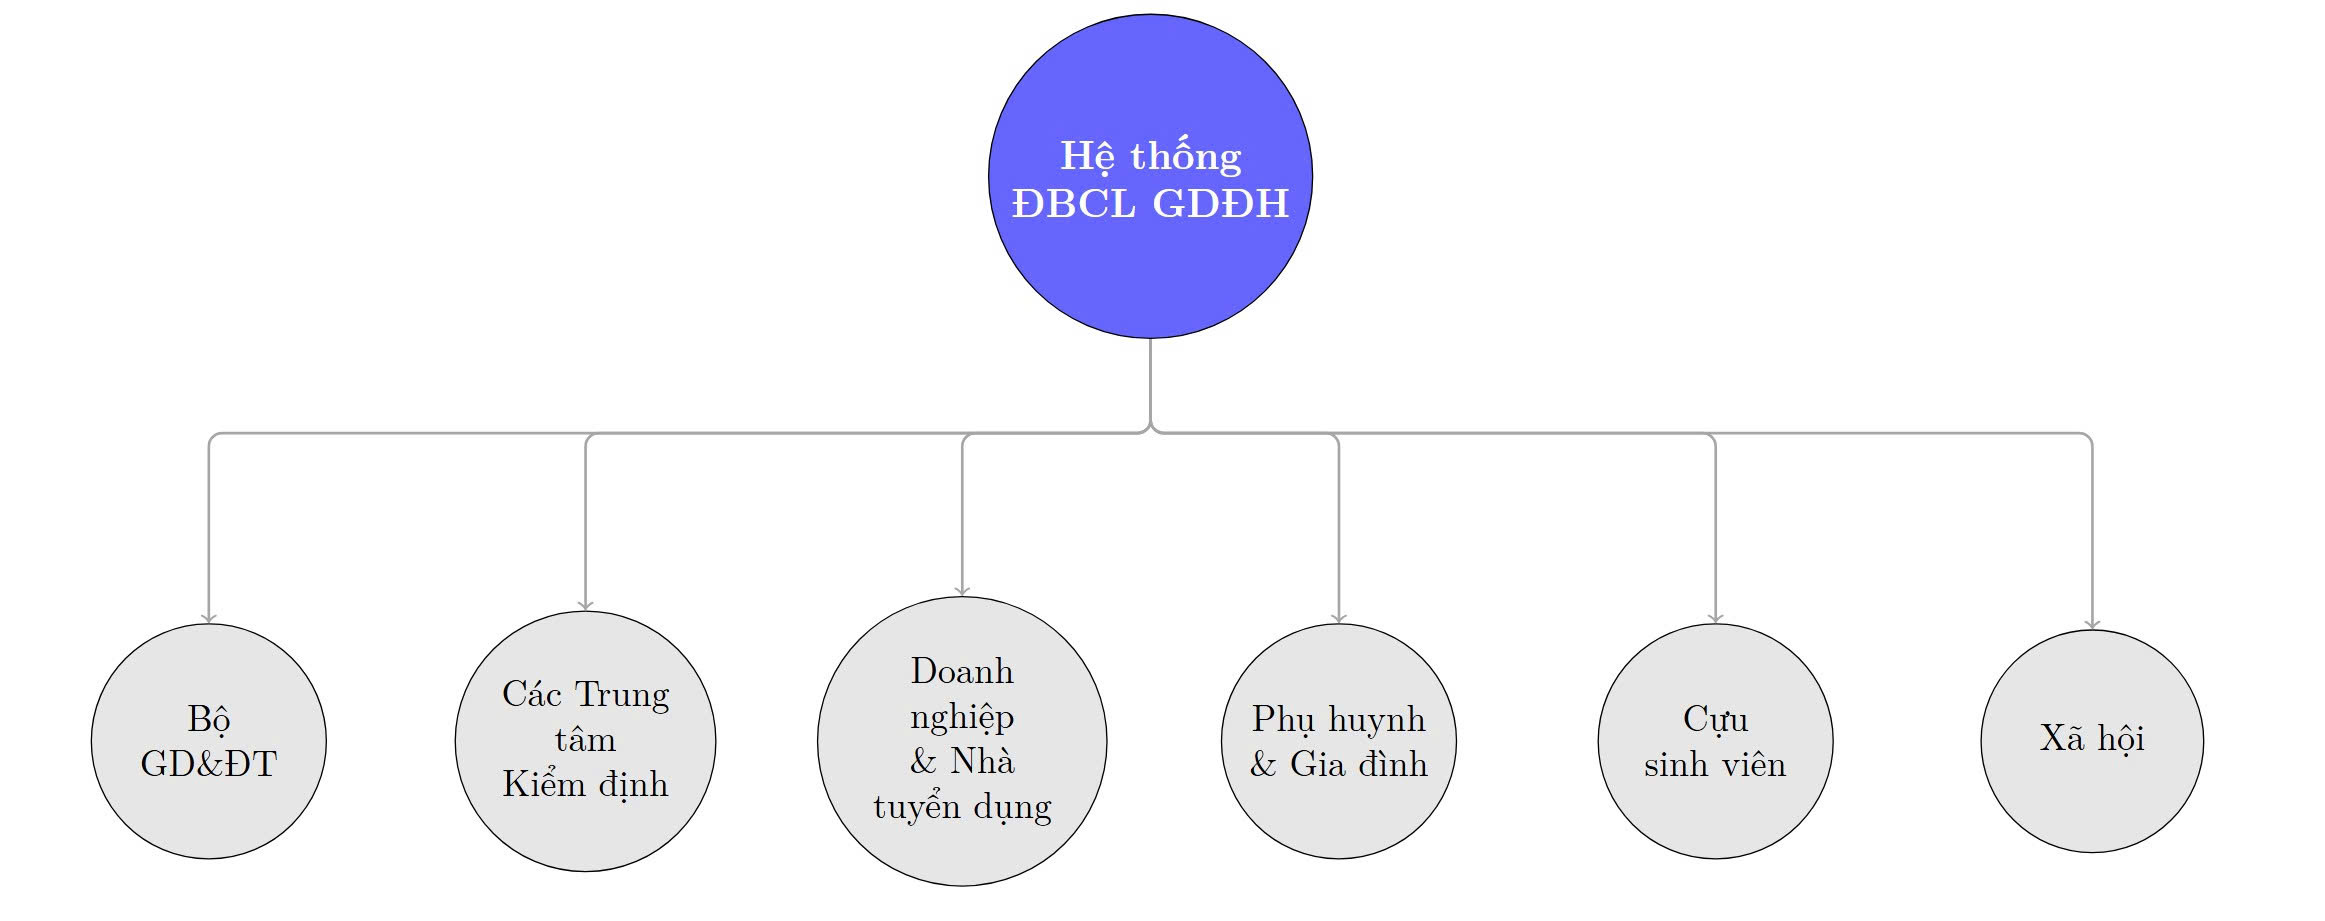
\includegraphics[width=\textwidth]{image/stakeholder_map.jpg} 
    \caption{越南高等教育质量保障体系中的利益相关者地图}
    \label{fig:stakeholder-map}
\end{figure}

\begin{itemize}
    \item \textbf{内部利益相关者 (Internal Stakeholders):}
        \begin{itemize}
            \item \textit{学校领导层(校董会、校领导班子):} 主要利益是学校的声誉、财务稳定、达成KPI指标以及遵守上级规定。
            \item \textit{教师与研究人员:} 利益包括学术自由、良好的工作条件、专业发展机会以及减少行政负担。
            \item \textit{行政人员(包括质量保障处干部):} 利益是流程清晰、有足够资源完成工作以及得到其他部门的合作。
            \item \textit{学生:} 核心利益是培养方案的质量、有效的教学方法、良好的学习环境、毕业后的就业机会以及合理的学费。
        \end{itemize}
    \item \textbf{外部利益相关者 (External Stakeholders):}
        \begin{itemize}
            \item \textit{教育培训部:} 利益是确保高等教育体系稳定运行、质量均衡,满足国家经济社会发展目标,并向政府和社会履行问责。
            \item \textit{教育质量认证中心:} 利益是维持其组织的声誉、专业性和独立性;完成被赋予的认证任务。
            \item \textit{企业与雇主:} 利益是能够招聘到具备与工作要求直接匹配的技能和知识的人力资源,减少再培训成本。
            \item \textit{家长与家庭:} 利益是为子女的投资(时间、金钱)带来应有的回报(孩子有好工作、成才)。
            \item \textit{校友:} 利益是学位证书的价值和母校声誉的提升,从而在职业网络中产生自豪感和机会。
            \item \textit{社会:} 利益是高等教育有助于创造一个公平、进步的社会,提供高质量的人力资源并维护文化价值观。
        \end{itemize}
\end{itemize}
该地图显示,质量保障体系必须服务于一个极其多样化的利益网络。一个质量改进的决策,例如增加学生的实践要求,可能会受到企业的欢迎,但却可能遭到教师(因工作量增加)或财务部门(因成本增加)的反对。识别和分析这些潜在的利益冲突,是构建一个有效的质量保障体系的第一步。



% done chuong 2 goi 2


% ======================================================================
% TRANG 11-13: THUYẾT CÁC BÊN LIÊN QUAN (PHẦN 2)
% ======================================================================

\subsubsection{利益相关者的显著性 (Stakeholder Salience)}

识别利益相关者仅仅是第一步。治理中的一个巨大挑战是如何处理来自这些群体的多样且常常相互矛盾的要求。并非所有利益相关者都具有同等的影响力。Mitchell, Agle和Wood(1997)提出了一个极具影响力的模型,用以确定利益相关者的“显著性”(salience),该模型基于三个核心属性\footcite{Mitchell1997}:

\begin{enumerate}
    \item \textbf{权力 (Power):} 利益相关者将其意志强加于组织之上的能力,迫使组织去做那些若无此压力则不会做的事情。权力可以来自对关键资源(如预算)的控制、颁布法规的能力或影响媒体的能力。
    \item \textbf{合法性 (Legitimacy):} 社会承认某一利益相关者的要求或行动在特定社会背景下是正当、适宜和正确的。合法性来自法律规定、合同或社会道德规范。
    \item \textbf{紧迫性 (Urgency):} 利益相关者的要求需要立即关注的程度。紧迫性取决于两个因素:时间敏感性(若不及时处理,要求将失去价值)和该要求对利益相关者的重要程度。
\end{enumerate}

根据拥有一、二或全部三个属性,利益相关者可被划分为不同优先级的群体,从“潜在”群体(latent stakeholders,仅有1个属性)到需要领导层最多关注的“决定性”群体(definitive stakeholders,拥有全部3个属性)。

将此模型应用于越南高等教育的质量保障体系,我们可以解释一些重要现象:
\begin{itemize}
    \item \textbf{教育培训部}是一个“决定性”利益相关者。该部拥有\textit{权力}(通过分配预算、颁发许可),拥有\textit{合法性}(依据《高等教育法》),并且其要求通常具有\textit{紧迫性}(与认证、报告周期挂钩)。因此,该部的声音分量最重,各大学通常优先满足其要求。
    \item \textbf{企业/雇主}是一个拥有\textit{合法性}(他们有权要求高质量的人力资源)和\textit{紧迫性}(人力需求不断变化)的利益相关者,但却缺乏直接\textit{权力}来迫使大学立即改变培养方案。这解释了为什么尽管企业不断抱怨学生质量,但大学培养方案的变革仍然缓慢。
    \item \textbf{学生和家长}拥有很高的\textit{合法性}和\textit{紧迫性},但他们的权力是分散的。只有当他们的要求通过大规模调查或媒体汇集起来时,他们的权力才会变得更加显著。
\end{itemize}
因此,显著性模型帮助我们理解,质量保障过程并非一个所有声音都平等的绝对民主过程,而是一个“政治舞台”,各大学必须不断权衡并优先考虑来自最具影响力的利益相关者的要求。

\subsubsection{利益相关者理论的应用与批判}

利益相关者理论提供了一个有效的分析工具,用以解读质量保障体系中的利益冲突。它有助于回答“质量为谁服务?”这一问题。通过识别利益相关者并分析其优先级,我们可以理解为什么质量的某些方面(例如:国际论文发表数量)会比其他方面(例如:学生的实践技能)更受重视。

然而,该理论也有其局限性。应用它时最大的挑战在于,当利益相互冲突时,如何找到一个最优方案来\textbf{平衡}这些利益。例如,为满足企业要求而加强实践教学会增加培养成本,可能导致学费上涨,从而引起学生和家长的反对。利益相关者理论很好地描述了这场争论,但并未提供解决它的明确公式。此外,该理论侧重于有形的关系和利益,但较少关注对组织行为有强大影响的无形文化规则和规范——而这正是新制度主义理论的长处。要理解具体的问责机制,我们需要借助第三种理论。

\subsection{委托代理理论 (Principal-Agent Theory)}
\label{subsec:uy_nhiem_nen_tang}

\subsubsection{起源与核心概念}
委托代理理论起源于经济学,特别是金融经济学和公司理论,其基础性工作由Stephen Ross等学者,特别是Michael Jensen和William Meckling在1970年代完成\footcite{JensenMeckling1976}。该理论旨在分析在一方(委托人 - Principal)雇佣或委托另一方(代理人 - Agent)代其执行某项工作时所产生的问题。

这种关系的核心问题(代理问题)源于两个基本条件:
\begin{enumerate}
    \item \textbf{目标冲突 (Conflict of Interest):} 委托人和代理人的利益并非总是一致。例如,股东(委托人)希望最大化利润,而管理者(代理人)可能希望最大化权力或其他个人利益。
    \item \textbf{信息不对称 (Information Asymmetry):} 代理人通常比委托人拥有更多关于工作及自身努力的信息。委托人难以完美地监督代理人的每一个行动。
\end{enumerate}
这两个条件的结合产生了两种主要风险\footcite{Eisenhardt1989}:
\begin{itemize}
    \item \textbf{道德风险 (Moral Hazard):} 合同签订后,由于委托人无法观察其努力程度,代理人可能不会尽全力工作。例如,一所大学(代理人)在从政府(委托人)获得预算后,可能不会尽最大努力投入于改进教学质量。
    \item \textbf{逆向选择 (Adverse Selection):} 签订合同前,代理人可能隐瞒信息或歪曲自身能力以求被选中。例如,一所大学可能会“美化”其自评报告,以获得认证机构的承认。
\end{itemize}
为解决这些问题,该理论提出了设计有效合同、创建激励机制(incentives)以协调利益等解决方案,最重要的是,建立\textbf{监督与报告系统(monitoring and reporting systems)}以减少信息不对称。


% done chuong 2 goi 3


% ======================================================================
% TRANG 16-18: THUYẾT ỦY NHIỆM (PHẦN 2) VÀ PHÊ PHÁN
% ======================================================================

\subsubsection{作为监督和合同机制的质量保障体系}

从委托代理理论的视角来看,整个外部质量保障体系可以被视为一个复杂的监督和合同机制,旨在解决“代理问题”。

\paragraph{多层次的委托代理关系:}
在高等教育中,关系不仅仅是单个委托人与代理人之间的关系。它是一系列相互嵌套的委托代理关系链,使得管理和监督变得复杂\footcite{Borgos2013}。我们可以将越南的这一关系链想象如下:
\begin{itemize}
    \item \textbf{第一层(政府 $\rightarrow$ 教育培训部):} 政府(委托人)将管理和发展国家高等教育体系的任务交给教育培训部(代理人)。
    \item \textbf{第二层(教育培训部 $\rightarrow$ 大学):} 教育培训部(委托人)向各大学(代理人)颁发办学许可并分配预算,期望各大学能够培养出高质量的人力资源并执行服务社会的研究任务。
    \item \textbf{第三层(校领导班子 $\rightarrow$ 院/系):} 校领导班子(委托人)将招生指标和预算分配给各院系(代理人),要求各院系保证其单位的培养和研究质量。
    \item \textbf{第四层(院/系 $\rightarrow$ 教师):} 院长/系主任(委托人)将教学任务分配给每位教师(代理人),并期望他们能以最佳方式完成授课。
\end{itemize}
这一委托代理链的存在解释了为什么来自最高层(政府)的要求在传达到下层时常常会被“干扰”或变形。

\paragraph{质量保障实践中的监督机制:}
为了在上述关系链中最大限度地减少道德风险和逆向选择,质量保障体系发展出了多种具体的监督机制:
\begin{itemize}
    \item \textbf{报告系统 (Reporting Systems):} 自评报告、年度报告、数据统计等要求,正是上级委托人收集下级代理人活动信息的工具。
    \item \textbf{外部认证 (External Accreditation):} 这是一种专门且正式的监督形式。认证机构(如VNU-CEA或AUN-QA)扮演着第三方“审计员”的角色,受委托人(教育培训部)信任,以核实信息并评估各大学(代理人)的活动\footcite{Borgos2013}。这一过程显著减少了信息不对称。
    \item \textbf{基于成果的合同 (Outcome-based Contracts):} 尽管在越南尚不普遍,但世界范围内的趋势是将预算分配与具体的产出结果(例如:学生就业率、国际发表数量)挂钩。这是一种旨在协调委托人与代理人利益的合同形式。
    \item \textbf{声誉建设 (Reputation Building):} 排名系统和公开认证结果也是一种监督机制。一所学校(代理人)的声誉成为一项重要资产,为了保护这项资产,他们有动力按照各委托人(学生、社会)的期望行事。
\end{itemize}

\subsubsection{委托代理理论的应用与批判}

委托代理理论提供了一套锐利的分析工具,用以剖析质量保障体系中的问责结构和监督机制。它逻辑地解释了为何需要报告、检查、定期认证等流程。特别是在分析合同性关系,如国家与被赋予自主权的公立大学之间的关系时,它尤其有用。

然而,机械地将委托代理理论应用于高等教育领域也有其显著的局限性\footcite{RIHE2022}:
\begin{itemize}
    \item \textbf{过分简化目标:} 该理论假设委托人的目标可以被明确定义。但在高等教育中,“质量”是一个多维度且难以衡量的概念。政府的目标可能是发展经济,而社会的目标是公平,学术界的目标则是创作自由。谁才是真正的“委托人”?
    \item \textbf{忽略文化与规范因素:} 该理论认为主体之间的关系主要基于经济利益和理性计算。它无法解释信任、共同价值观以及职业规范(例如:教师道德)在调节教师和学校行为中的作用。
    \item \textbf{难以应用完美的合同:} 在现实中,很难设计一个能预见所有情况并准确衡量代理人所有努力的合同。教育的“产品”(人)是极其复杂的,不能像工业产品那样容易衡量。
\end{itemize}
正因为这些局限性,分析质量保障体系不能仅仅依赖委托代理理论。必须将其与新制度主义理论(以理解无形规则)和利益相关者理论(以理解多样化利益)相结合,才能获得更全面、更准确的图景。

% ======================================================================
% TRANG 19-20: CÁC MÔ HÌNH ĐBCL HIỆN ĐẠI
% ======================================================================
\section{世界现代质量保障模型}
\label{sec:mo_hinh_hien_dai_the_gioi}

治理理论的发展和实践中的挑战,推动了日益精密的质量保障模型的诞生。这些模型不再固守单一理论,而是对传统方法的局限性进行综合和超越的努力。其中,混合模型和适应性框架这两个突出的趋势,对越南具有重要的参考意义\footcite{HybridModel2023}\footcite{AdaptiveQA2022}。

\subsection{混合模型 (Hybrid Model): 协调问责与改进}

\subsubsection{诞生背景与理念}
传统的质量保障体系通常陷入两个极端之一。一是,体系过分注重对外部的\textbf{问责制(accountability)}(自上而下),导致学校只专注于形式上、应付性地遵守规定,形成一种“合规文化”(culture of compliance)而非实质性改进。这是一种接近委托代理理论思维的模式。二是,体系过分注重\textbf{内部改进(improvement)}(自下而上),将全部权力交给单位自行评估,导致缺乏共同标准且难以确保对社会的问责。

混合模型应运而生,旨在解决这种紧张关系\footcite{EUA_Integration}。其理念是承认并整合这两个目标。它认为一个可持续的质量保障体系必须既能满足外部的控制和透明度要求,又能激发内部的改进动力和发展质量文化。混合模型不将问责与改进视为对立的目标,而是视其为一枚硬币的两面,相辅相成。例如,外部透明的问责要求可以为推动内部改进努力提供必要的数据和压力。反之,强大的内部改进文化将使学校更容易满足并超越外部的问责要求。

\subsubsection{组成部分与特点}
一个典型的混合模型通常具有以下特点:
\begin{itemize}
    \item \textbf{双重标准框架:} 体系可能包括一套用于问责目的的强制性\textbf{最低标准(minimum standards)},以及一套用于改进目的的鼓励性\textbf{提升标准(enhancement standards)}。
    \item \textbf{嵌套流程:} 外部认证活动的设计不仅旨在检查合规性,还旨在提供建设性建议,支持学校的改进过程。反之,内部自评和改进活动的结果被用作外部认证轮次中的重要证据。
    \item \textbf{质量保障机构的灵活角色:} 外部质量保障机构不仅扮演“裁判员”的角色,还扮演“伙伴”、“顾问”的角色,在改进过程中为学校提供支持。
\end{itemize}
欧洲质量保障体系的经验,尤其是在博洛尼亚进程之后,显示出向混合模型转变的明显趋势,其中认证流程越来越被设计为服务于质量提升的目标(enhancement-led accreditation)\footcite{EUA_Integration}。越南的实践,既要满足教育培训部的国家标准,又要参与如AUN-QA等区域认证项目,也正显示出一种混合模型正在逐渐形成的迹象,尽管可能尚非完全自觉\footcite{VNU-CEA2023}\footcite{HangNguyen2017}。

% done chuong 2 goi 4



% ======================================================================
% TRANG 21-22: KHUNG THÍCH ỨNG
% ======================================================================

\subsection{适应性框架 (Adaptive Framework): 在变化世界中的质量管理}
\label{subsec:khung_thich_ung}

\subsubsection{与传统方法的比较}
如果说混合模型解决了质量保障\textit{目标}的矛盾,那么适应性框架则解决了在不稳定和复杂环境中\textit{实施流程}的问题。传统的项目管理方法,通常被称为“瀑布模型”(Waterfall Model),遵循一个严格的线性序列:规划 → 设计 → 执行 → 测试 → 交付。该模型假设所有要求和条件都可以从一开始就明确确定,并且在整个过程中环境不会改变。

然而,在高等教育的现实中,尤其是在越南,情况则完全不同。教育部的政策可能改变,劳动力市场的需求波动,教育技术发展迅速,学校的资源也不稳定。采用一个僵化的、长达5年的瀑布式质量保障计划,通常会导致计划在尚未执行完毕时就已经过时。

适应性框架(Adaptive Framework),其源于敏捷软件开发(Agile)领域,正是为了解决这些问题而生\footcite{Wysocki2009}。它不是试图从一开始就制定一个完美的计划,而是将项目分解为短期的、重复的周期。在每个周期结束时,项目团队将重新评估结果,收集反馈,并为下一个周期调整计划。

\subsubsection{适应性框架的核心原则}
一个具有适应性的质量保障框架将基于以下原则运作:
\begin{itemize}
    \item \textbf{迭代学习 (Iterative Learning):} 整个质量保障流程被视为一个学习过程。学校可以不必每5年进行一次大型评估,而是可以针对具体方面(如教学方法、学生服务)进行更小规模的评估周期(例如,每年一次)。每个周期的结果将为改进下一个周期提供信息。
    \item \textbf{反馈循环 (Feedback Loops):} 该框架创建了快速且频繁的反馈循环。学校不必等到5年周期结束才有认证报告,而是可以在每学期或每学年后与学生、教师和企业组织反馈会议。
    \item \textbf{增量发展 (Incremental Development):} 质量改进不必同时进行,而是可以分阶段、逐步实施。例如,第一年,学校可以集中改进学生意见收集系统;第二年,专注于创新学习成果评估方法。
    \item \textbf{价值驱动的优先级排序 (Value-driven Prioritization):} 在每个周期,改进活动将根据其在当时为最重要利益相关者带来的价值来进行优先排序。
\end{itemize}

\subsubsection{对越南国情的适用性}
认为适应性框架特别适合越南国情的论点基于以下原因:
\begin{itemize}
    \item \textbf{动态的政策环境:} 越南关于高等教育的法规和政策可能会迅速变化。一个适应性框架允许学校灵活调整其质量保障策略,以适应新的要求,而无需推翻整个旧计划。
    \item \textbf{资源限制:} 学校不必投入巨额资金进行全面改革,而是可以根据其在每个阶段的有限资源,进行小规模、渐进式的改进。
    \item \textbf{逐步建立能力:} 立即实施一个复杂的质量保障体系可能会给人力团队带来过重负担。适应性框架允许学校边做边学,逐步且可持续地建立质量保障能力。
\end{itemize}
因此,将混合模型的理念与适应性框架的流程相结合,将创造出一种在目标上全面、在实施方式上灵活且务实的质量保障方法。这正是为越南构建建议模型的基础。

% ======================================================================
% TRANG 23-25: ĐỀ XUẤT MÔ HÌNH V-AQA
% ======================================================================
\section{为越南高等教育提出分析模型:混合与适应性模型 (V-AQA)}
\label{sec:mo_hinh_V-AQA_de_xuat}

\subsection{建立一个综合模型的必要性论证}
\label{subsec:luan_giai_V-AQA}
通过以上各部分的分析可以看出,使用单一理论来分析越南高等教育的质量保障体系是不全面的,并可能导致片面的结论。
\begin{itemize}
    \item \textbf{如果仅使用新制度主义},我们将能解释为何各学校会形式化地遵守规定,但难以解释来自内部的实质性改进努力或利益冲突。
    \item \textbf{如果仅使用利益相关者理论},我们将能看到利益多样化的图景,但却缺乏分析工具来解释为何某些方面的声音比其他方面更有分量,也无法解释报告和监督机制。
    \item \textbf{如果仅使用委托代理理论},我们将能清晰理解问责结构,但却会忽略文化、规范因素以及无法简化为单纯合同的复杂合作关系。
\end{itemize}

因此,越南的国情需要一个综合的分析框架,一个能够融合不同视角的模型。本论文提出了这样一个模型,名为\textbf{越南高等教育混合与适应性质量保障模型(The Vietnam - Adaptive Quality Assurance Model,简称 V-AQA)}。

该模型具有\textbf{混合性(Hybrid)},因为它承认并试图协调两个并行且时而矛盾的目标:
\begin{enumerate}
    \item \textbf{对外部的问责制(External Accountability):} 满足教育培训部、认证机构和社会的要求,以获得合法性和资源(反映了新制度主义和委托代理理论的视角)。
    \item \textbf{来自内部的改进(Internal Improvement):} 为内部利益相关者(学生、教师)创造价值,并推动一种内生的质量文化(反映了利益相关者理论的视角)。
\end{enumerate}

同时,该模型具有\textbf{适应性(Adaptive)},因为它在实施过程中强调灵活性,允许大学根据反馈和环境变化,以短期周期调整其质量保障活动,而不是遵循一个僵化的五年计划。

\subsection{V-AQA模型的结构与核心要素}
\label{subsec:cau_truc_V-AQA}

V-AQA模型的结构如同一座神殿,以理论为基石,以最终目标为屋顶,并由五个核心要素作为五根支柱支撑。这五个要素并非独立运作,而是相互作用、相互巩固,形成一个稳固的系统(见图 \ref{fig:v-aqa-model-detailed})。

\begin{figure}[h!]
    \centering
    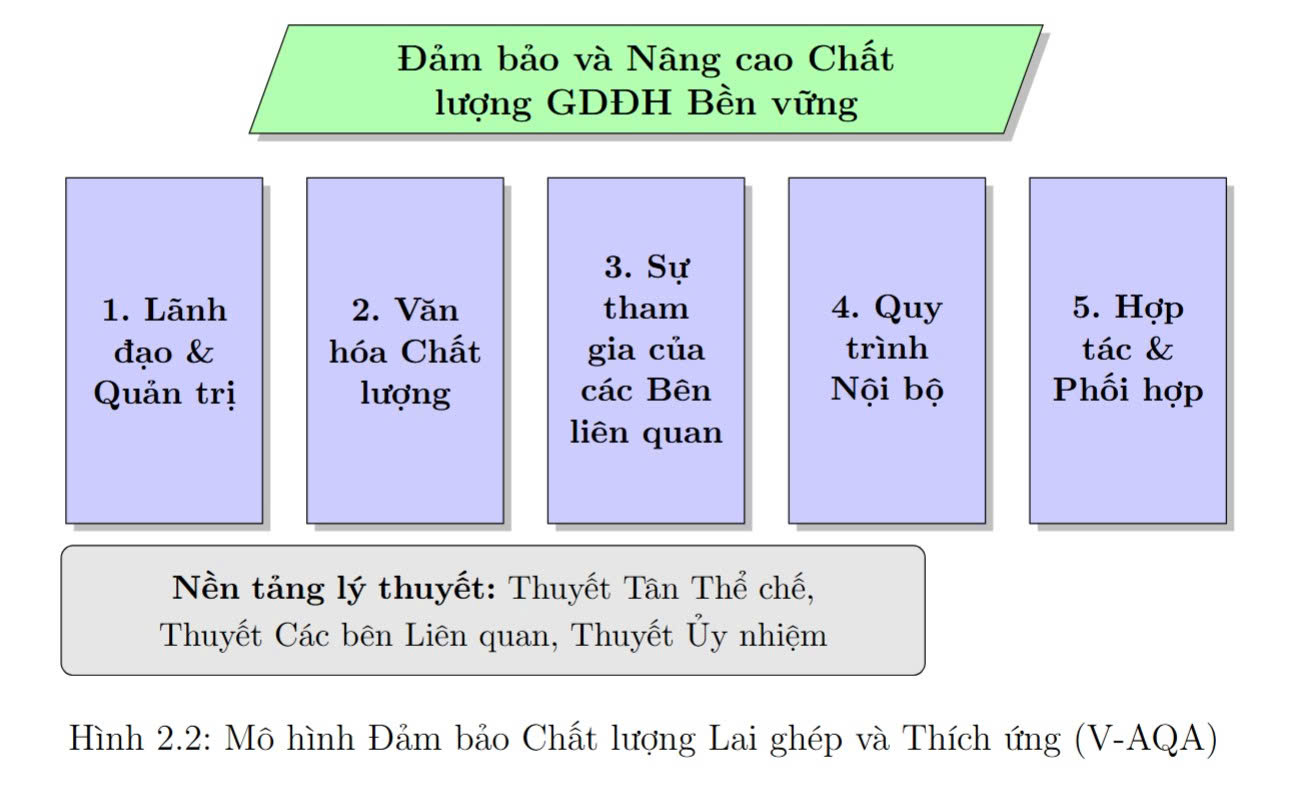
\includegraphics[width=0.9\textwidth]{image/mo_hinh_V-AQA.jpg}
    \caption{混合与适应性质量保障模型 (V-AQA)}
    \label{fig:v-aqa-model-detailed}
\end{figure}

\subsubsection{要素1的详细分析:领导与治理 (Leadership \& Governance)}
\label{subsubsec:thanh_to_1}

\paragraph{定义与范围:}
领导与治理要素是整个质量保障体系的源头,为之指明方向并提供资源。它不仅是行政管理活动,更是领导层在构建愿景、激发灵感以及建立有效治理结构以实现该愿景的能力。在越南的背景下,该要素包括校董会、校领导班子以及各级院、处、室领导的作用。它通过颁布关于质量的战略、政策及执行这些政策的承诺来体现。

\paragraph{理论与实践基础:}
该要素受到\textbf{委托代理理论}和\textbf{新制度主义理论}的强烈映射。
\begin{itemize}
    \item 从委托代理理论的角度看,学校领导层既是上级管理机构(教育培训部)的\textit{代理人},有责任执行国家政策;又是下级单位(院、系)的\textit{委托人},有责任监督并确保这些单位有效运作。明确的治理结构和责任划分是解决内部代理问题的先决条件。
    \item 从新制度主义的角度看,领导者是“解读”并诠释来自制度场域压力的角色。他们决定学校的战略:是被动遵守、模仿成功模式,还是主动寻求独特道路以创造差异化和独特的合法性。领导者的愿景将塑造学校与外部环境互动的方式。
\end{itemize}

\paragraph{实践中的指标与表现:}
为了评估一所大学在该要素上的发展水平,可以考察以下指标:
\begin{itemize}
    \item 是否存在一份详细的校级\textit{质量战略},并将其融入学校的总体发展战略中。
    \item 校领导班子、校董会涉及质量保障问题的会议频率和内容。
    \item 为质量保障活动分配资源(财务、人力)的程度。
    \item 规定质量保障相关单位职能、任务的文件的明确性。
    \item 关于干部、教师对领导层在质量工作中的承诺和导向作用的意见调查结果。
\end{itemize}
对这些指标的分析将在本论文的现状章节中详细进行。

% done chuong 2 goi 5


% ======================================================================
% TRANG 26-28: PHÂN TÍCH CHI TIẾT THÀNH TỐ 2: VĂN HÓA CHẤT LƯỢNG
% ======================================================================

\subsubsection{要素2的详细分析:质量文化 (Quality Culture)}
\label{subsubsec:thanh_to_2}

\paragraph{定义与范围:}
质量文化不仅是对质量的认知或口号,而是一个共享的价值观、信念、期望和承诺的集合,它塑造了一个教育机构中所有成员在保障和提升质量方面的行为\footcite{HarveyStensaker}。它是在谈论质量时“我们在这里做事的方式”(the way we do things around here)。该要素与“合规文化”(culture of compliance)相对立,在合规文化中,质量保障活动只是为了应付外部要求而机械地执行。

质量文化的范围非常广泛,它渗透到学术生活的每一个角落,从一名教师如何准备教案,一个院系如何组织专业研讨会,到学校领导层如何做出战略决策。一个强大的质量文化将把质量保障从一种行政负担转变为个人和组织发展的内在动力。

\paragraph{理论基础与质量文化的维度:}
质量文化通过\textbf{新制度主义理论}的视角得到最清晰的体现,特别是其\textit{规范性(normative)}和\textit{文化-认知性(cultural-cognitive)}两大支柱。
\begin{itemize}
    \item \textbf{规范性方面:} 质量文化通过职业规范形成和巩固。当“持续改进”或“以学习者为中心”成为学术界所重视的规范时,个人为了被视为专业的教育者和管理者,会倾向于按照该规范行事。
    \item \textbf{文化-认知性方面:} 质量文化作为一种无需思考即被接受的脚本或常识而存在。届时,收集学生反馈或定期审查培养方案不再是一项要求,而是一件“理所当然”必须做的事情。
\end{itemize}

为了系统地分析质量文化,可以使用Harvey和Stensaker(2008)的模型,该模型将质量文化分为四种类型,反映了组织的成熟度\footcite{HarveyStensaker}:
\begin{enumerate}
    \item \textbf{反应型文化 (Reactive Culture):} 组织仅在出现问题或有外部检查要求时才关注质量。这是最低的层次。
    \item \textbf{响应型文化 (Responsive Culture):} 组织开始建立流程和体系以响应质量要求,但动力主要仍来自外部。许多越南大学目前正处于此阶段,为应对认证评估而建立质量保障部门和流程。
    \item \textbf{再生/改进型文化 (Regenerative Culture):} 这是一个质的飞跃。组织有能力自我评估,自我发现问题,并主动实施持续改进的循环。改进的动力来自内部。
    \item \textbf{繁殖/传播型文化 (Reproductive Culture):} 在最高层次,组织不仅自我改进,还成为典范,向外传播关于质量的最佳实践,为其他组织塑造规范。
\end{enumerate}
该模型为诊断和确定一所大学质量文化的发展目标提供了有用的工具。

\paragraph{在越南实践中的指标与表现:}
质量文化是一个抽象的概念,但可以通过具体的指标和表现来间接衡量:
\begin{itemize}
    \item \textbf{领导层的承诺:} 公开发言、战略文件以及资源分配是否显示出质量保障是真正的优先事项。
    \item \textbf{教师和员工的态度:} 关于工作满意度、对质量保障活动(视其为负担还是机遇)的态度的调查结果,以及自愿参与改进活动的程度。
    \item \textbf{内部使用的语言:} 内部文件和会议是使用“遵守”、“响应要求”的语言,还是“提升”、“改进”、“卓越”的语言?
    \item \textbf{认可与奖励机制:} 学校是否有机制来表彰和奖励有质量改进创举的个人和单位?
\end{itemize}
正如专家报告所反映的,越南的现状表明,许多大学仍在努力从“响应型”文化向“改进型”文化转型。来自认证评估的压力通常会产生临时性的活动,质量文化尚未真正深入到每位教师的日常工作中\footcite{ExpertPerspectivesVN}\footcite{CommonFailureCriteria}。这是V-AQA模型需要解决的最大挑战之一。

% ======================================================================
% TRANG 29-30: PHÂN TÍCH CHI TIẾT THÀNH TỐ 3: SỰ THAM GIA CỦA CÁC BÊN LIÊN QUAN
% ======================================================================

\subsubsection{要素3的详细分析:利益相关者的参与 (Stakeholder Engagement)}
\label{subsubsec:thanh_to_3}

\paragraph{定义与范围:}
利益相关者的参与不仅仅是“征求意见”或“举办研讨会”。它是一个有系统的、有目的的过程,旨在将利益相关者吸引到质量保障的各个环节中,从培养方案的设计,到教与学的过程,再到评估和改进。这是“质量为谁服务?”这一理念的实现,承认一个高质量的培养方案必须为不同的对象群体创造价值。

参与的范围很广,包括从低到高的多种形式:
\begin{itemize}
    \item \textbf{告知 (Informing):} 向利益相关者单向提供信息。
    \item \textbf{咨询 (Consulting):} 征求利益相关者的意见和反馈。
    \item \textbf{卷入 (Involving):} 在整个过程中与利益相关者直接合作。
    \item \textbf{协作 (Collaborating):} 在决策中成为合作伙伴。
    \item \textbf{授权 (Empowering):} 将最终决策权交给利益相关者。
\end{itemize}
一个成熟的质量保障体系需要根据具体问题和具体利益相关者,为不同层次的参与提供机制\footcite{Arnstein1969}。

\paragraph{理论与实践基础:}
该要素是\textbf{利益相关者理论}的直接应用。它将重心从一个封闭、内向的管理模式转向一个开放、外向的模式。这也是混合模型的一个核心要素,因为正是来自外部利益相关者的反馈和要求,构成了内部改进活动的重要动力。

国际实践,特别是欧洲的经验表明,利益相关者,尤其是学生和雇主的参与,是现代质量保障体系中不可或`缺的要素。像AUN-QA这样的标准体系也对在审查和改进培养方案中收集和使用利益相关者反馈提出了明确要求\footcite{ENQA_Stakeholder2018}\footcite{AUN-QAGuide}。

\paragraph{在越南实践中的指标与表现:}
该要素的发展水平可以通过以下指标进行评估:
\begin{itemize}
    \item \textbf{有外部人员参与的委员会的存在:} 例如,科学与培养委员会、每个专业的行业咨询委员会(Industry Advisory Board)。
    \item \textbf{咨询活动的频率和实质性:} 与雇主举行的研讨会数量、校友调查、为学生设立的反馈渠道。
    \item \textbf{影响的证据:} 是否有具体证据表明培养方案已根据企业或校友的反馈进行了调整和更新。
    \item \textbf{学生在各委员会中的角色:} 学生在院级、校级委员会中是否有代表,他们的声音是否得到实质性的倾听和记录。
\end{itemize}
在越南,这是仍存在诸多局限的要素之一。报告通常指出,校企联系仍然松散且形式化。培养方案的制定通常主要基于学术团队的观点,而很少有雇主的实质性参与\footcite{CommonFailureCriteria}。因此,加强利益相关者的参与是越南高等教育质量保障体系改革的一个重要方向。

% done chuong 2 goi 6


% ======================================================================
% TRANG 31-35: PHÂN TÍCH CHI TIẾT THÀNH TỐ 4: QUY TRÌNH NỘI BỘ
% ======================================================================

\subsubsection{要素4的详细分析:内部流程 (Internal Processes)}
\label{subsubsec:thanh_to_4}

\paragraph{定义与范围:}
如果说前面的要素关注的是“为什么”(理论)、“谁”(领导者、利益相关者)和“什么”(文化),那么要素4则关注\textbf{“如何做?”}的问题。内部流程是一所教育机构用来系统地管理核心学术活动以保障和提升质量的一整套标准化的政策、程序、指南和工具。

这是质量保障体系的“运行机器”,将质量战略和目标转化为具体且可衡量的行动。该要素的范围涵盖了学生的整个学术生命周期,从培养方案的设计到学生毕业并由雇主评估。在本论文的框架内,我们将重点关注三个最重要的子流程:(1)培养方案(CDĐT)的设计与审查;(2)教-学活动与评估的管理;以及(3)数据收集与分析系统。

\paragraph{子流程4.1:培养方案(CDĐT)的设计与审查}
这是决定学校所提供的教育“产品”的基础流程。一个有效的流程必须确保培养方案既具科学性,又能满足利益相关者的需求。

\textit{理论基础:} 该流程是三大基础理论的交汇点。\textbf{利益相关者理论}要求流程必须有机制来收集和整合来自学生、企业的要求。\textbf{新制度主义理论}解释了为什么培养方案通常必须遵守教育培训部颁布的“课程框架”(强制性同形),并倾向于参考知名大学(模仿性同形)。\textbf{委托代理理论}将培养方案视为学校(代理人)承诺为社会和国家(委托人)执行的一种详细“合同”。

\textit{标准流程中的步骤:} 一个有效的培养方案设计与审查流程通常包括以下步骤,正如AUN-QA等国际标准所建议的\footcite{AUN-QAGuide}:
\begin{enumerate}
    \item \textbf{确定预期学习成果(Expected Learning Outcomes - ELOs):} 这是最重要的一步。ELOs必须基于与利益相关者(特别是雇主)的协商来制定,必须清晰、可衡量,并与学校的使命和愿景相符。
    \item \textbf{构建课程地图(Curriculum Mapping):} 设计课程和学习活动,使其能够逻辑地、系统地为实现既定的ELOs做出贡献。该技术有助于确保整个方案的一致性和建设性对齐(constructive alignment)。
    \item \textbf{审批与颁布:} 必须有一个科学与培养委员会(有外部专家参与)在正式颁布前对培养方案进行审定和批准。
    \item \textbf{定期审查与改进:} 必须有一个定期流程(例如:每2-3年一次),根据来自校友、雇主的反馈、学生的学习成果以及行业的新趋势来重新审查培养方案。
\end{enumerate}

\textit{越南现状:} 这是仍然存在许多薄弱环节的领域之一。认证报告通常指出,许多学校的培养方案设计流程仍然是封闭的,主要依赖于教师团队的经验,而缺乏企业的实质性参与。课程审查通常没有系统地进行,导致培养方案落后于劳动力市场的要求\footcite{CommonFailureCriteria}。

\paragraph{子流程4.2:教-学活动与评估的管理}
如果说培养方案是“设计图”,那么这就是“施工”过程。教-学活动和评估的质量直接决定了学生的学习体验和学习成果。

\textit{理论基础:} \textbf{委托代理理论}解释了监督教学活动(听课、检查)的必要性,以减少道德风险(教师备课不认真)。\textbf{利益相关者理论}强调了学生通过调查系统对教学质量提供反馈的作用。

\textit{流程的组成部分:}
\begin{itemize}
    \item \textbf{教学管理流程:} 包括关于制定详细课程大纲、准备教案、应用积极教学方法以及听课、向教师提建议的机制的规定。
    \item \textbf{学生学习成果评估流程:} 需要多样化评估形式,不仅仅依赖期末考试。过程性评估、项目、演讲、团队合作以及基于实践能力的测试等形式需要被标准化并广泛应用。必须有建立试题库、出题、阅卷和复核的透明、公平的流程。
    \item \textbf{反馈流程(Feedback):} 必须有机制让学生定期对每门课程和教师提出反馈。更重要的是,必须有流程来处理这些反馈,并向学生通报已进行的改变和改进。
\end{itemize}

\textit{越南现状:} 这也是一个固有的弱点。认证报告经常指出,单向讲授法被滥用,评估方法主要依赖记忆,以及来自学生的反馈系统仍然是形式化的,并未真正影响到教学的改进\footcite{ExpertPerspectivesVN}\footcite{CommonFailureCriteria}。

\paragraph{子流程4.3:数据收集与分析系统 – 基于证据的治理基础}

这是整个质量保障体系的“神经系统”,是支持其他流程的最重要的技术要素。没有它,所有改进决策都有可能变得主观和缺乏依据。

\textit{理论基础与作用:} 该系统是\textbf{委托代理理论}中监督机制的实现,是倾听\textbf{利益相关者}声音的工具,也是\textbf{新制度主义理论}下专业化、合理化的一个象征。它使学校能够从基于经验的管理模式转向基于证据的治理(evidence-based governance)。

\textit{核心功能:}
\begin{enumerate}
    \item \textbf{收集 (Collection):} 建立流程,从多个来源(学生学习成果、招生数据、教师人事信息、满意度调查结果、校友就业数据、财务数据等)一致地、定期地收集数据。
    \item \textbf{管理 (Management):} 构建一个集中的数据库(database)或数据仓库(data warehouse)来存储、清理和管理已收集的数据。
    \item \textbf{分析 (Analysis):} 使用统计和分析工具将原始数据转化为有意义的信息。例如:寻找教学方法与学生学习成果之间的相关性,或分析影响学生辍学率的因素。
    \item \textbf{报告与可视化 (Reporting \& Visualization):} 构建自动化的报告(reports)和仪表盘(dashboards)系统,直观地为不同级别的管理层提供信息,以支持决策。
\end{enumerate}

\textit{越南现状:} 这被认为是越南质量评估报告中最大和最普遍的挑战\footcite{CommonFailureCriteria}\footcite{AUN-QA_Challenges_VN}。学校通常缺乏一个集成的数据系统;数据分散在不同的部门,没有标准化,难以利用。决策通常仍然更多地依赖于领导的经验,而不是客观的数据分析。构建这样一个系统需要对技术和人力进行大量投资,这是一个巨大的障碍。

\paragraph{关于内部流程要素的结论:}
这三个子流程相互之间联系紧密。一个设计良好的培养方案(4.1)如果不能通过有效的教-学和评估方法(4.2)来实施,将毫无意义。而要知道流程(4.1)和(4.2)是否有效,学校需要一个强大的数据系统来衡量和分析(4.3)。任何一个流程的薄弱都会影响到整个系统。因此,标准化和改进这些内部流程是任何质量保障努力的核心任务。

% done chuong 2 goi 7

% ======================================================================
% TRANG 36-37: PHÂN TÍCH CHI TIẾT THÀNH TỐ 5: HỢP TÁC & PHỐI HỢP
% ======================================================================

\subsubsection{要素5的详细分析:合作与协调 (Cooperation \& Collaboration)}
\label{subsubsec:thanh_to_5}

\paragraph{定义与范围:}
在V-AQA模型中,合作与协调不仅是一项临时性的活动,而是一个战略性要素,是组织的核心能力。它被定义为一所教育机构打破“孤岛”(silos)以在不同个人、单位和组织之间创造联系和协同效应(synergy),从而实现共同质量目标的能力。该要素的范围包括三个层面:
\begin{itemize}
    \item \textbf{内部合作 (Internal Cooperation):} 同一所大学内部各院、处、室、中心之间的协调。例如:教务处、质量保障处与各专业院系在审查培养方案中的协调。
    \item \textbf{校际合作 (Inter-institutional Cooperation):} 国内各大学之间的合作,通过质量标杆比对(benchmarking)、经验分享、建立联合培养项目或关于质量保障的联合研究项目等活动进行。
    \item \textbf{国际合作 (International Cooperation):} 学校参与区域和国际质量保障网络(如AUN-QA),与国外大学合作,或邀请国际专家参与咨询和认证委员会。
\end{itemize}

\paragraph{理论与实践基础:}
该要素由三大基础理论共同诠释:
\begin{itemize}
    \item 从\textbf{新制度主义理论}的角度看,合作与组织网络是规范性同形和模仿性同形最重要的传播渠道。当各大学相互合作时,它们学习并应用最佳实践,逐渐为整个行业形成一套共同的规范。参与国际网络也有助于学校增强其在国际舞台上的合法性。
    \item 从\textbf{利益相关者理论}的角度看,合作正是最高层次的参与形式。它不止于倾听,而是共同行动。当校企关系是一种战略合作关系,双方共同参与设计和实施培养方案时,这种关系将最为有效。
    \item 从\textbf{委托代理理论}的角度看,合作可以被视为一种有助于减少信息不对称和监督成本的机制。例如,一个由多所学校组成的网络共同参与同行评审(peer review),将创造出比每所学校单独报告更有效、更可靠的监督机制。
\end{itemize}

\paragraph{在越南实践中的指标与表现:}
该要素的发展水平可以通过以下方面来衡量:
\begin{itemize}
    \item \textbf{内部层面:} 是否存在跨院系的委员会或项目;各职能部门在质量保障活动中的协调程度。
    \item \textbf{校际层面:} 国内各校之间的合作协议、联合培养项目或关于质量保障的联合研究成果的数量。
    \item \textbf{国际层面:} 在国际网络中的成员数量;由外国组织认证的专业数量;邀请国际专家参与学术和质量保障活动的频率。
\end{itemize}
越南的实践表明,尽管一些顶尖大学正在大力推动国际合作和参与AUN-QA网络,但单位之间的内部合作以及国内各大学之间的系统性合作仍然存在诸多局限。打破“部门壁垒”和“本位主义”思维仍然是构建一个真正质量生态系统的巨大挑战。

% ======================================================================
% TRANG 38-40: PHÂN TÍCH SỰ TƯƠNG TÁC VÀ VẬN HÀNH CỦA MÔ HÌNH V-AQA
% ======================================================================
\subsection{V-AQA模型的互动与运作分析}
\label{subsec:tuong_tac_V-AQA}

以上提出的五个要素并非五个独立、零散的因素。V-AQA模型的优势和力量正是在于它们之间的\textbf{动态互动和系统性}。仅仅关注一个或两个要素而忽略其他要素,将无法创造一个可持续的质量保障体系。例如,一所学校可能在纸面上有非常好的内部流程(要素4),但如果缺乏领导层的承诺(要素1)和积极的质量文化(要素2),这些流程将只会被形式化地执行。

为了说明该模型的运作,我们可以想象一个在实践中典型的质量改进循环(见图\ref{fig:v-aqa-cycle})。

\begin{figure}[h!]
    \centering
    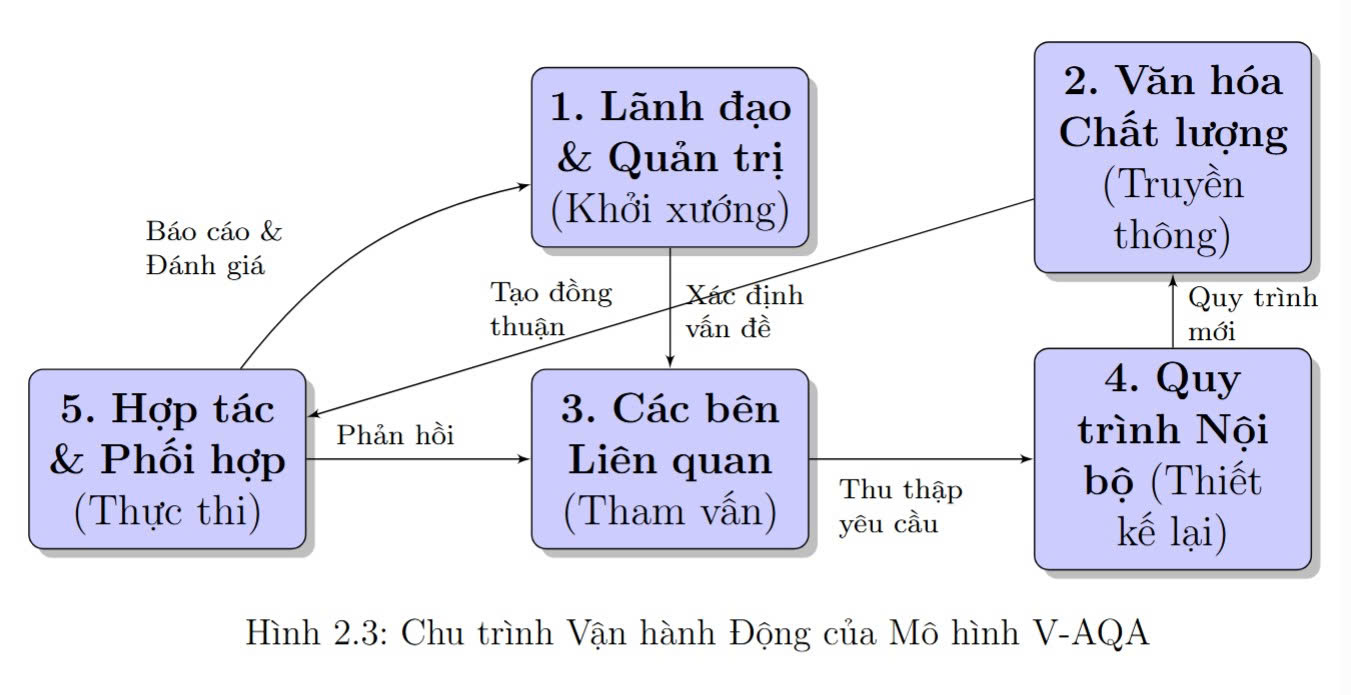
\includegraphics[width=0.9\textwidth]{image/chu_trinh_van_hanh_V-AQA.jpg}
    \caption{V-AQA模型的动态运作循环}
    \label{fig:v-aqa-cycle}
\end{figure}


一个改进循环可能如下进行:
\begin{enumerate}
    \item \textbf{从领导层发起:} 循环始于\textbf{领导与治理(要素1)}识别出一个紧迫的质量问题,这可能来自外部压力(教育培训部的新要求)或内部数据(毕业生就业率低)。领导层做出需要变革的战略决策。
    \item \textbf{咨询利益相关者:} 领导层不是自行提出解决方案,而是发起一个与\textbf{利益相关者(要素3)}的咨询过程。成立一个工作组,包括企业代表、校友、教师和学生,以收集多维度的要求和视角。
    \item \textbf{重新设计内部流程:} 基于咨询结果,相关的\textbf{内部流程(要素4)}(例如:培养方案设计流程)被重新设计,以整合新的要求。
    \item \textbf{建立文化与合作:} 这个新流程随后在全校范围内广泛沟通,以形成共识并建立\textbf{质量文化(要素2)}。实施过程需要各院系和职能部门之间紧密的\textbf{合作与协调(要素5)}。
    \item \textbf{反馈与适应循环:} 实施一段时间后,数据系统(属于要素4)将收集新的结果。这些结果被分析并报告给领导层(要素1)。基于这份报告,领导层将评估变革的效果,并为新的周期决定下一步的改进措施。
\end{enumerate}
该循环清晰地体现了模型的\textbf{混合性}和\textbf{适应性}。它之所以是\textit{混合的},因为它平衡了来自外部的合规压力(领导层发起)和为利益相关者创造价值的需求(咨询)。它之所以是\textit{适应性的},因为它不是一次性的过程,而是一个持续的循环,允许学校学习并调整其战略。这是彼得·圣吉(Peter Senge)观点下的“学习型组织”(learning organization)的一种方法,在这种组织中,成员不断扩展其能力以创造他们真正期望的结果\footcite{Senge2006}。

这种系统性方法需要一种新的治理思维,超越管理孤立的部门,而专注于管理它们之间的关系和信息流。这既是挑战,也是在越南建立一个真正有效和可持续的质量保障体系的关键。

% done chuong 2 goi 8















